\subsection{Изоморфные графы}

\begin{defn}
    Графы $G_1 = \langle V_1, E_1 \rangle$ и $G_2 = \langle V_2, E_2 \rangle$ изоморфны, если существует биекция $f : V_1 \to V_2$ такая, что любых двух вершин $u, v \in V_1$ они смежны тогда и только тогда, когда $f(u)$ и $f(v)$ смежны.
\end{defn}

\begin{center}
    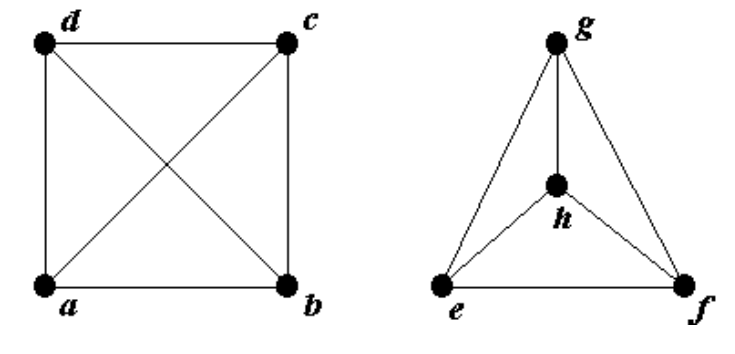
\includegraphics[width=0.5\textwidth]{par25izo.png}
\end{center}

$f : a \to e,~b \to f,~c \to g,~d \to h$

\begin{statement}
    Два графа изоморфны $\iff$ вершины одного из них можно перенумеровать, так чтобы матрица смежности этого графа совпала с матрицей смежности второго графа.
\end{statement}